\documentclass[12pt]{article}
\usepackage[utf8]{inputenc}
\usepackage{graphicx}
\usepackage{caption}
\usepackage{float}
\usepackage[a4paper, top=3cm, bottom=3cm, left=4cm, right=3cm]{geometry}
\usepackage{fancyhdr}
\usepackage{fontspec}
\usepackage{array}
\usepackage{longtable}
\usepackage{etoolbox}
\usepackage{setspace}
\usepackage{titlesec}

\setmainfont{Times New Roman}

% --- SPASI NASKAH 1.5 & PARAGRAF ---
\setstretch{1.5}
\setlength{\parindent}{1.27cm}
\setlength{\parskip}{12pt}

% --- FORMAT SUBBAB (Font 12pt BOLD, Ukuran Standar) ---
\titleformat{\section}{\normalfont\bfseries}{\thesection}{1em}{}
\titlespacing*{\section}{0pt}{2pt}{-6pt}

% --- NAMA & PENOMORAN LANGSUNG (TANPA CHAPTER) ---
\renewcommand{\figurename}{Gambar}
\renewcommand{\tablename}{Tabel}

% Format angka dipaksa diawali 4.x
\renewcommand{\thetable}{4.\arabic{table}}
\renewcommand{\thefigure}{4.\arabic{figure}}

\setcounter{table}{4}   % Tabel pertama otomatis jadi 4.5
\setcounter{figure}{91} % Gambar pertama otomatis jadi 4.92

% --- FORMAT CAPTION ---
\captionsetup[figure]{labelfont=bf, textfont=normalfont, labelsep=space, justification=centering}
\captionsetup[table]{labelfont=bf, textfont={normalfont, stretch=1}, labelsep=space, justification=raggedright, singlelinecheck=false, skip=0pt, margin=0pt, indention=0pt}

% --- KHUSUS LONGTABLE (Font 10pt & Spasi 1.0) ---
\AtBeginEnvironment{longtable}{\singlespacing\fontsize{10}{12}\selectfont}
\setlength{\LTpre}{0pt}
\setlength{\LTpost}{0pt}

% --- NOMOR HALAMAN 145 KANAN ATAS ---
\setcounter{page}{145}
\pagestyle{fancy}
\fancyhf{}
\renewcommand{\headrulewidth}{0pt}
\fancyhead[R]{\thepage}

\begin{document}

\section*{4.3 \textit{Lighthouse Testing}}

\sloppy

\textit{Lighthouse testing} dilakukan untuk mengukur kualitas aplikasi web secara keseluruhan, khususnya dalam memenuhi standar PWA. Pengujian ini mencakup 4 metrik utama: \textit{Performance}, \textit{Accessibility}, \textit{Best Practices}, dan SEO. Pengujian dilakukan pada halaman utama aplikasi (\textit{dashboard}) menggunakan \textit{DevTools Lighthouse} bawaan \textit{browser}. Ringkasan hasil pengujian dapat dilihat pada Tabel \ref{tab:pengujian-lighthouse} berikut.

\captionsetup[longtable]{justification=raggedright, singlelinecheck=false}
\setlength{\LTcapwidth}{11cm}
\addtolength{\LTcapwidth}{8\tabcolsep}
\addtolength{\LTcapwidth}{5\arrayrulewidth}
\begin{longtable}{|>{\centering\arraybackslash}p{1cm}|p{4.5cm}|>{\centering\arraybackslash}p{2.5cm}|>{\centering\arraybackslash}p{3cm}|}
\caption{Tabel Hasil \textit{Lighthouse Testing}} \label{tab:pengujian-lighthouse} \\
\hline
\textbf{No} & \textbf{Kategori Metrik} & \textbf{Skor} & \textbf{Status} \\ \hline
\endfirsthead
\hline
\textbf{No} & \textbf{Kategori Metrik} & \textbf{Skor} & \textbf{Status} \\ \hline
\endhead
\hline
\endfoot
1 & \textit{Performance} & 97 & Baik \\ \hline
2 & \textit{Accessibility} & 100 & Baik \\ \hline
3 & \textit{Best Practices} & 100 & Baik \\ \hline
4 & SEO & 100 & Baik \\ \hline
\end{longtable}

\begin{figure}[H]
    \centering
    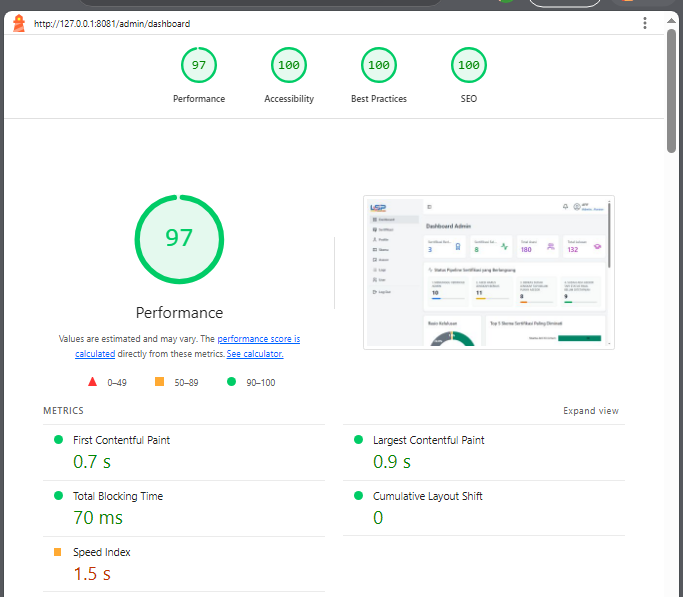
\includegraphics[width=\textwidth]{images/lighthouse-test.png}
    \caption{Hasil \textit{Lighthouse testing}}
    \label{fig:lighthouse-test}
\end{figure}

\end{document}